% AVATIC workshop presentation (INFINIUM '26)
% Build:  cd workshop && latexmk -pdf presentation.tex      (or: pdflatex presentation.tex, twice)
%
% ---------------------------------------------------------------------------
% EDIT HERE: dates and prizes (shown on several slides)
\newcommand{\RoundOneOpens}{TBA}          % simulation round opens
\newcommand{\RoundOneDeadline}{TBA}       % simulation submission deadline
\newcommand{\ShortlistDate}{TBA}          % shortlist for the hardware round announced
\newcommand{\RoundTwoDate}{TBA}           % hardware round (on site)
\newcommand{\PrizePool}{To be announced}
\newcommand{\ContactName}{Srinath Bhamidipati}
\newcommand{\ContactMail}{srinath.bhamidipati@research.iiit.ac.in}
\newcommand{\RepoURL}{github.com/Srindot/AVATIC}
% ---------------------------------------------------------------------------

\documentclass[aspectratio=169,11pt]{beamer}
\usetheme{Madrid}
\usepackage[T1]{fontenc}
\usepackage{graphicx}
\usepackage{booktabs}
\usepackage{tabularx}
\usepackage{tikz}
\usetikzlibrary{arrows.meta,positioning,shapes.geometric,fit,calc}
\usepackage{fontawesome5}

% colours
\definecolor{avBlue}{RGB}{21,67,122}
\definecolor{avAccent}{RGB}{230,120,20}
\definecolor{bGreen}{RGB}{13,166,26}
\definecolor{bBlue}{RGB}{13,64,230}
\definecolor{bYellow}{RGB}{242,204,13}
\definecolor{bRed}{RGB}{217,13,13}
\setbeamercolor{structure}{fg=avBlue}
\setbeamercolor{palette primary}{bg=avBlue,fg=white}
\setbeamercolor{palette secondary}{bg=avBlue!80!black,fg=white}
\setbeamercolor{palette tertiary}{bg=avBlue!60!black,fg=white}
\setbeamercolor{frametitle}{bg=avBlue,fg=white}
\setbeamercolor{title}{bg=avBlue,fg=white}
\setbeamercolor{block title}{bg=avBlue,fg=white}
\setbeamercolor{block body}{bg=avBlue!6}
\setbeamercolor{block title alerted}{bg=avAccent,fg=white}
\setbeamercolor{block body alerted}{bg=avAccent!8}
\setbeamertemplate{navigation symbols}{}
\setbeamertemplate{itemize items}[circle]

% helpers
\newcommand{\balloon}[1]{\tikz[baseline=-0.6ex]\fill[#1] (0,0) ellipse (0.13 and 0.17);}
\newcommand{\code}[1]{\texttt{\small #1}}
% an image, or a labelled placeholder box if the file is not there yet
\newcommand{\figOrBox}[3]{% #1 file, #2 width, #3 label
  \IfFileExists{#1}{\includegraphics[width=#2]{#1}}{%
    \tikz\node[draw=avBlue,dashed,thick,minimum width=#2,minimum height=0.56*#2,
      align=center,text width=#2-6mm,font=\scriptsize,text=avBlue]{\faImage[regular]\\ #3};}}

\title[AVATIC]{AVATIC}
\subtitle{Autonomous Vision-Based Aerial Target Interception Challenge}
\author[INFINIUM '26]{INFINIUM '26 \quad\textbullet\quad Workshop}
\institute[]{\RepoURL}
\date{}

\begin{document}

% ===========================================================================
\begin{frame}
  \titlepage
  \vspace{-4mm}
  \begin{center}
    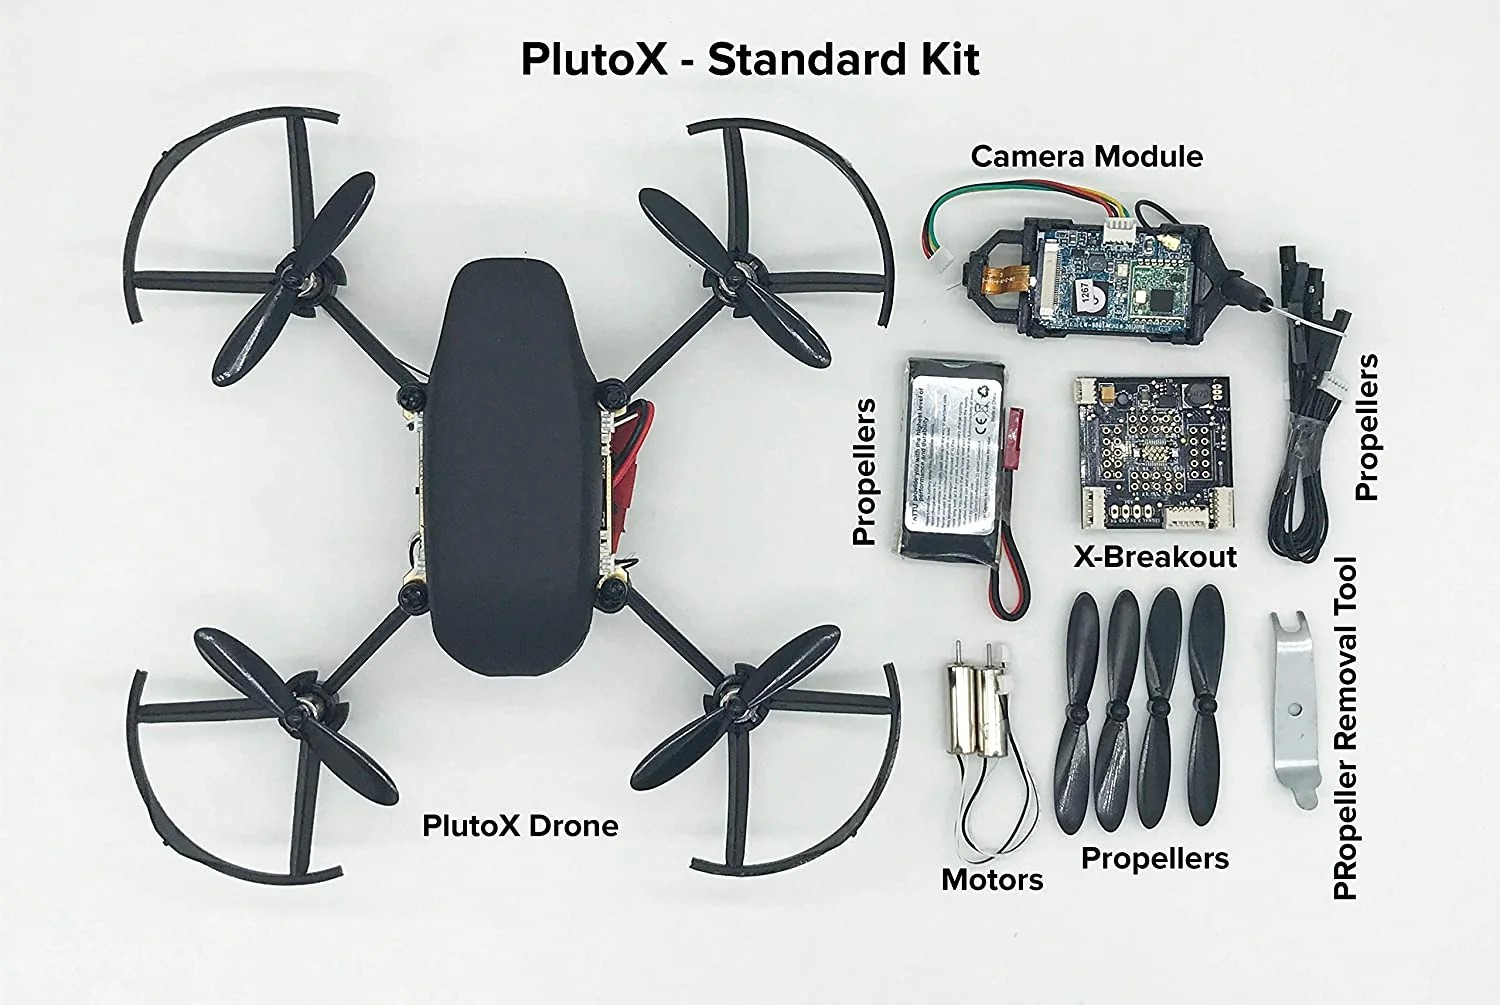
\includegraphics[height=0.26\textheight]{figures/pluto_x.jpg}\hspace{4mm}
    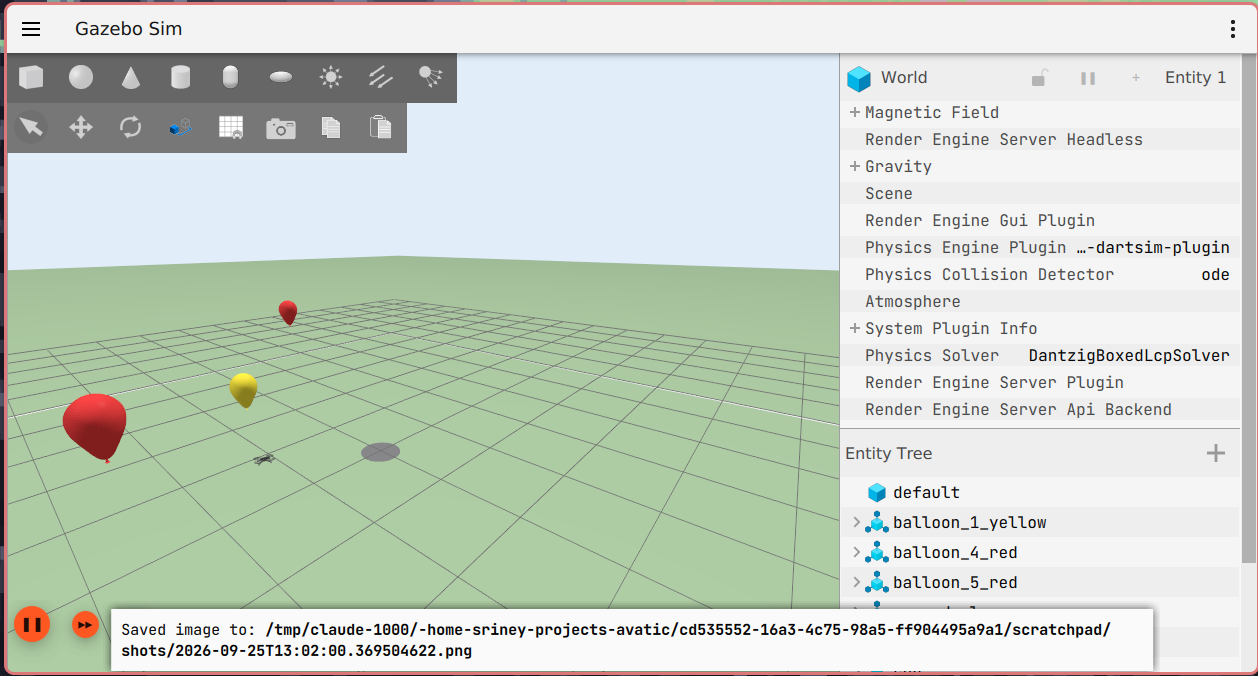
\includegraphics[height=0.26\textheight]{figures/simulation.png}
  \end{center}
\end{frame}

\begin{frame}{Today}
  \begin{columns}[T]
    \column{0.5\textwidth}
    \begin{enumerate}
      \item The objective
      \item Game rules: balloons and points
      \item Overview: the drone, the simulator, the two rounds
      \item Rounds, deadlines and what we expect
      \item The simulation round in depth
    \end{enumerate}
    \column{0.5\textwidth}
    \begin{enumerate}\setcounter{enumi}{5}
      \item Solution ideas (a starting point, not a solution)
      \item Sim2real: from the simulator to the real Pluto X
      \item Deadlines, once more
      \item Prizes
      \item Questions
    \end{enumerate}
  \end{columns}
\end{frame}

% ===========================================================================
\section{Objective}
\begin{frame}{The objective}
  \begin{columns}[c]
    \column{0.55\textwidth}
    \begin{block}{Your mission}
      Write a program that flies a \textbf{Pluto X} drone into balloons
      using \textbf{only its camera}.
    \end{block}
    \begin{itemize}
      \item Your algorithm runs on \textbf{your laptop}.
      \item It receives the \textbf{video from the drone}, decides how to fly,
            and sends \textbf{flight commands} back.
      \item Pop the good balloons, avoid the red ones, in \textbf{15 seconds}.
      \item No GPS, no position, no map: just the camera and the drone's
            own readings (tilt, heading, height).
    \end{itemize}
    \column{0.43\textwidth}
    \centering
    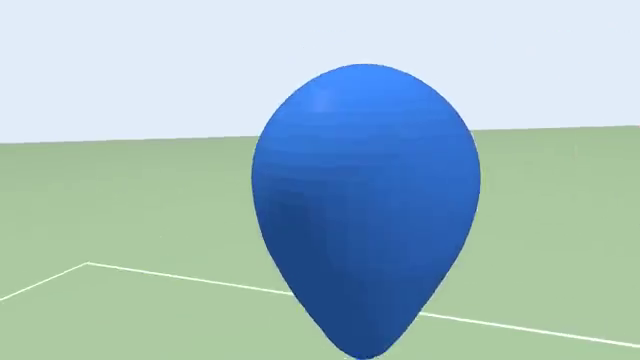
\includegraphics[width=\linewidth]{figures/cam_prepop.png}\\[1mm]
    {\scriptsize What your program sees, just before a pop}
  \end{columns}
\end{frame}

% ===========================================================================
\section{Game rules}
\begin{frame}{Game rules: balloons and points}
  \begin{columns}[c]
    \column{0.48\textwidth}
    \centering
    \renewcommand{\arraystretch}{1.5}
    \begin{tabular}{clrc}
      \toprule
      & \textbf{Balloon} & \textbf{Points} & \textbf{How many} \\
      \midrule
      \balloon{bGreen}  & green  & \textbf{+100} & 2 \\
      \balloon{bBlue}   & blue   & \textbf{+50}  & 3 \\
      \balloon{bYellow} & yellow & \textbf{+25}  & 4 \\
      \balloon{bRed}    & red    & \textcolor{bRed}{\textbf{$-$75}} & 3 \\
      \bottomrule
    \end{tabular}\\[3mm]
    \textbf{Best possible score: 450}
    \column{0.5\textwidth}
    \begin{itemize}\small
      \item \textbf{12 balloons}, the more points the rarer; 30\,cm wide,
            0.8--2\,m high, 1--3.5\,m from the start
      \item more good balloons than anyone can pop: \textbf{choose well}
      \item a balloon \textbf{pops when the drone touches it}
      \item \textbf{15 s} from arming; later pops don't count
      \item red \textbf{costs points}: the score can go negative
      \item the drone starts facing east: balloons are often \textbf{behind} it
      \item \textbf{random layouts}: judging uses layouts nobody has seen
    \end{itemize}
  \end{columns}
\end{frame}

% ===========================================================================
\section{Overview}
\begin{frame}{Overview: two rounds, one program}
  \centering
  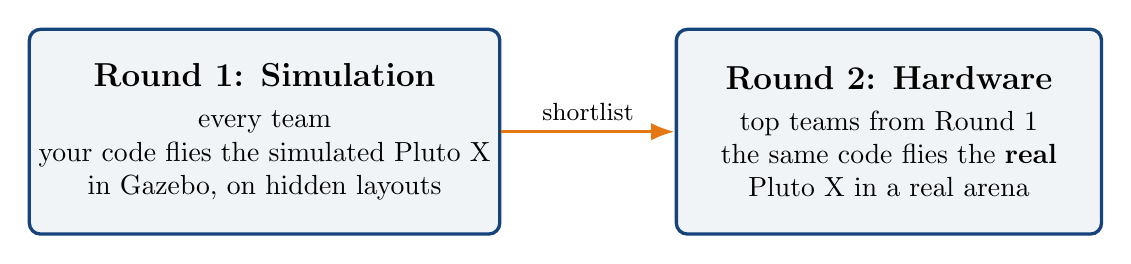
\begin{tikzpicture}[
      box/.style={draw=avBlue,very thick,rounded corners,fill=avBlue!6,
                  minimum width=5.4cm,minimum height=2.6cm,align=center},
      arr/.style={-{Latex[length=3mm]},very thick,avAccent}]
    \node[box] (r1) {\textbf{\large Round 1: Simulation}\\[1mm]
      every team\\ your code flies the simulated Pluto X\\ in Gazebo, on hidden layouts};
    \node[box,right=2.2cm of r1] (r2) {\textbf{\large Round 2: Hardware}\\[1mm]
      top teams from Round 1\\ the same code flies the \textbf{real}\\ Pluto X in a real arena};
    \draw[arr] (r1) -- node[above,font=\small,text=black]{shortlist} (r2);
  \end{tikzpicture}\\[4mm]
  \begin{columns}[c]
    \column{0.45\textwidth}\centering
    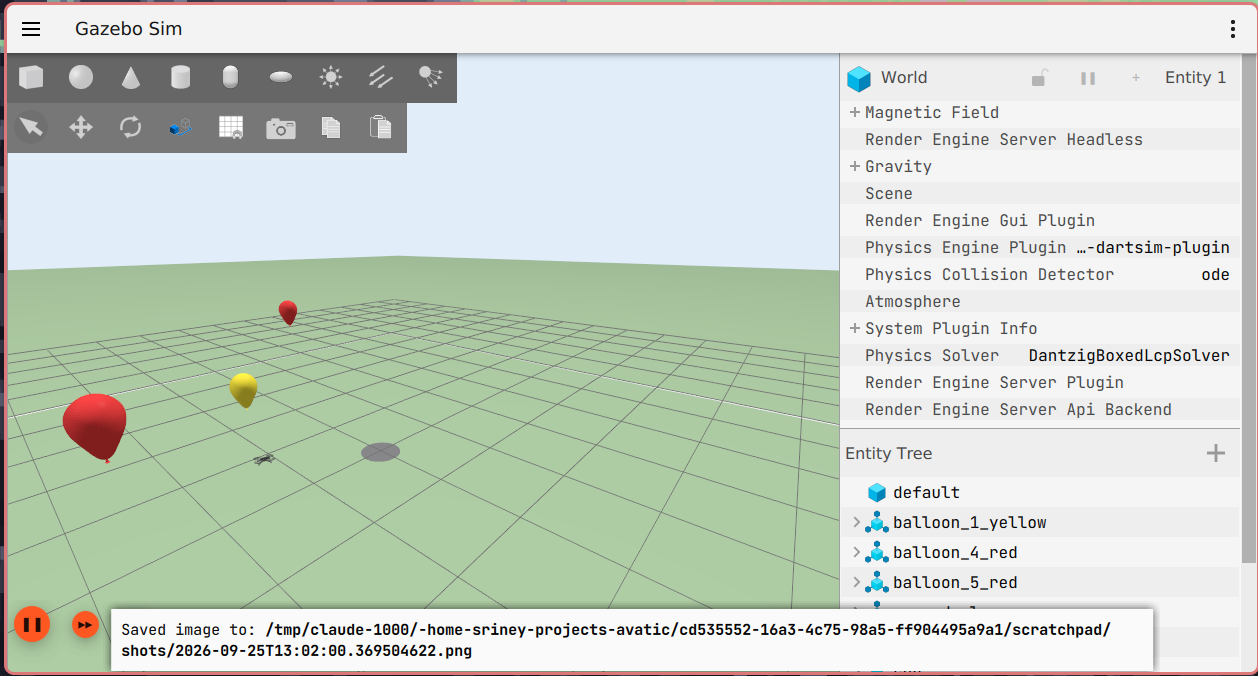
\includegraphics[width=0.85\linewidth]{figures/simulation.png}\\
    {\scriptsize The simulated arena (Gazebo)}
    \column{0.45\textwidth}\centering
    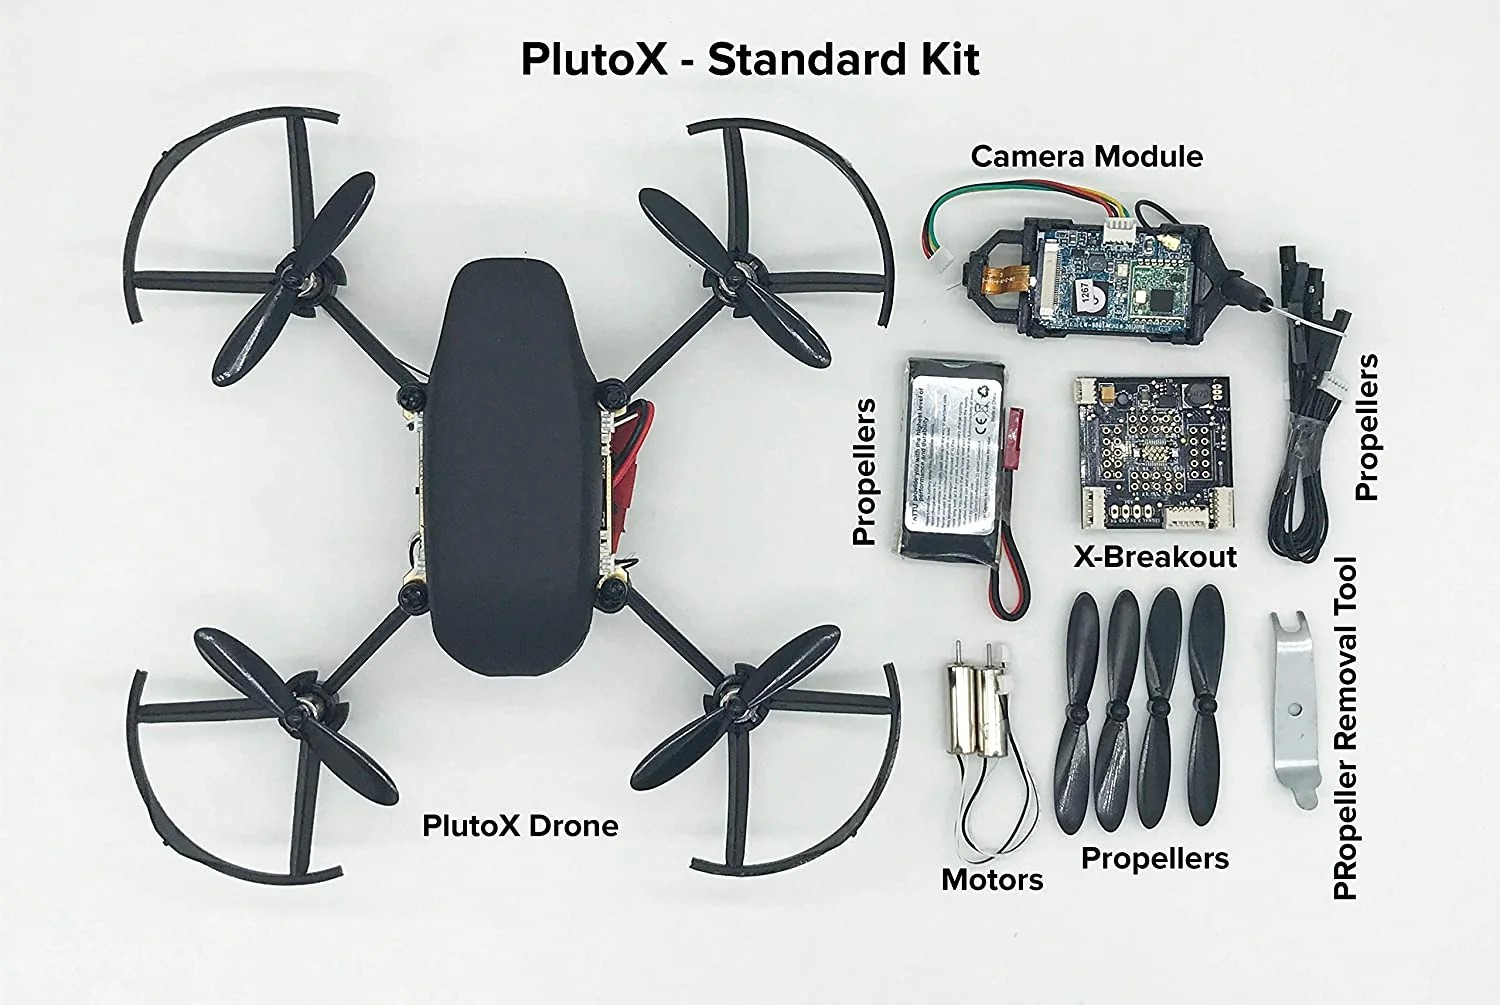
\includegraphics[width=0.75\linewidth]{figures/pluto_x.jpg}\\
    {\scriptsize The real Pluto X kit}
  \end{columns}
\end{frame}

\begin{frame}{The hardware: Pluto X}
  \begin{columns}[c]
    \column{0.42\textwidth}
    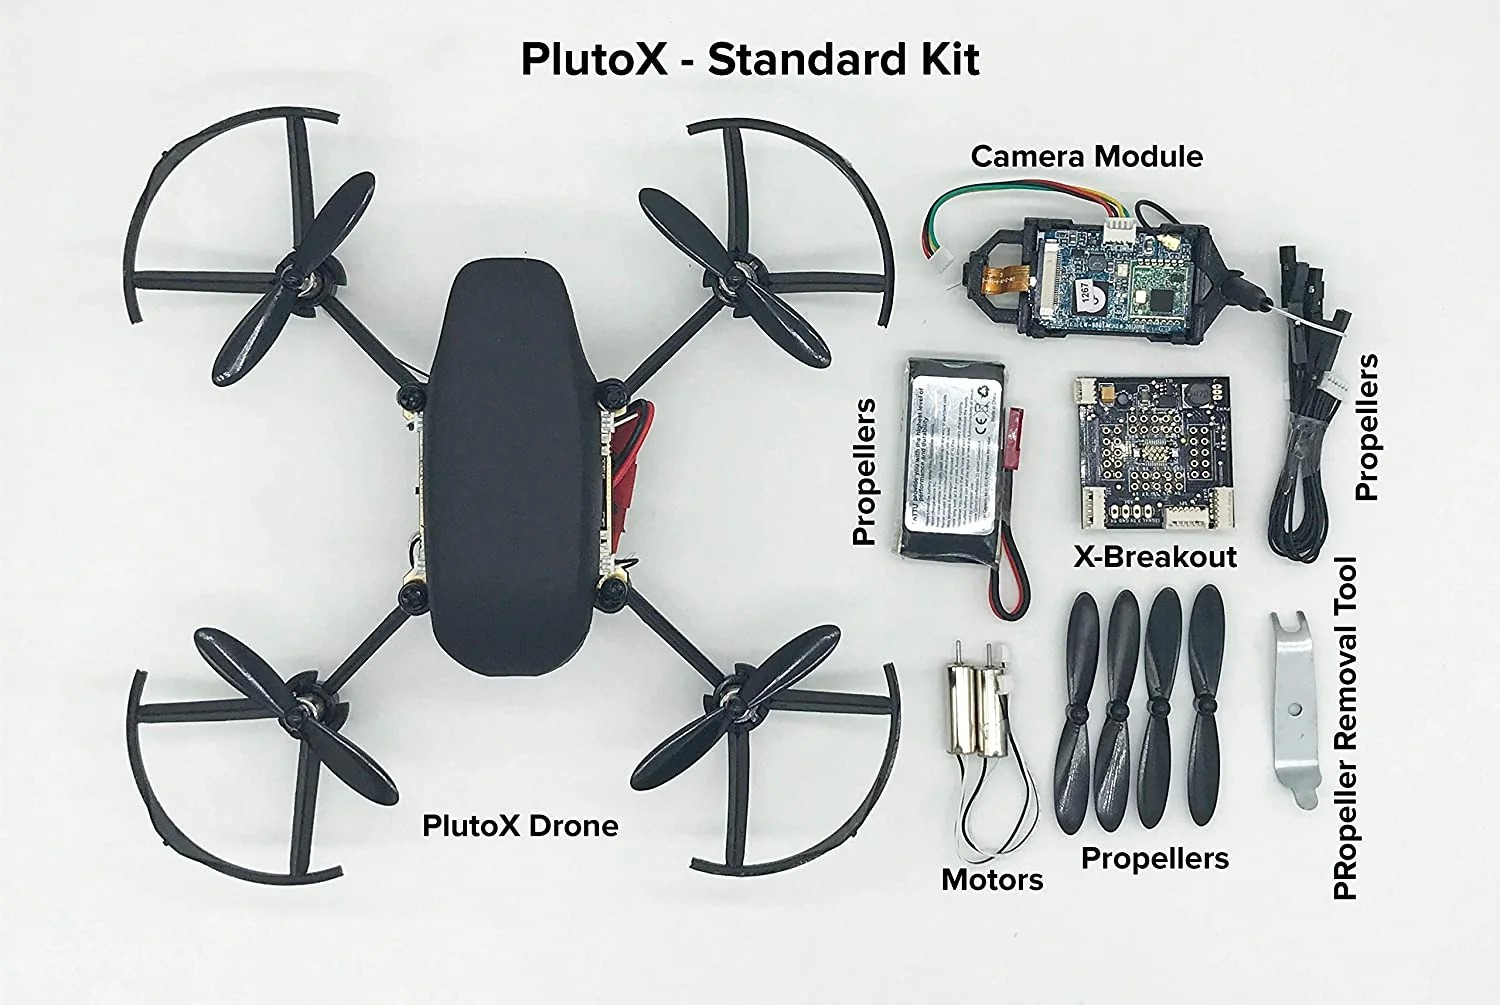
\includegraphics[width=\linewidth]{figures/pluto_x.jpg}
    \column{0.56\textwidth}
    \scriptsize
    \renewcommand{\arraystretch}{1.15}
    \begin{tabularx}{\linewidth}{@{}lX@{}}
      \toprule
      Maker & Drona Aviation \\
      Size, weight & 16 $\times$ 16 $\times$ 4\,cm, 68\,g with the camera \\
      Motors & 4 brushed coreless, 55\,mm propellers \\
      Battery & 1S LiPo 3.7\,V, 600\,mAh (about 9 min) \\
      Flight controller & STM32F303 running \textbf{MagisV2} firmware \\
      Sensors & ICM-20948 (gyro, accel, magnetometer), ICP-10111 barometer \\
      Camera & 1280 $\times$ 720, about 18 fps over Wi-Fi, $\approx$80° field of view \\
      Link & Wi-Fi to your laptop (MSP protocol) \\
      \midrule
      You read & tilt, heading, barometric height, battery, armed \\
      You send & roll, pitch, yaw rate, throttle \\
      \bottomrule
    \end{tabularx}
  \end{columns}
\end{frame}

\begin{frame}{The simulation stack}
  \begin{columns}[c]
    \column{0.52\textwidth}
    \begin{itemize}
      \item \textbf{Gazebo Harmonic}: physics and the 3-D world
      \item \textbf{ROS 2 Humble}: plumbing between the parts
            (hidden from you)
      \item The drone's \textbf{real MagisV2 firmware}, running
            unmodified in the loop
      \item Simulated \textbf{sensors} with realistic noise: gyroscope,
            accelerometer, magnetometer, barometer, battery, camera
      \item \textbf{Wind gusts}, command delay, motor lag, air drag,
            battery sag
      \item Scoring, recording of every run, analysis and evaluation
            tools
    \end{itemize}
    \column{0.46\textwidth}
    \centering
    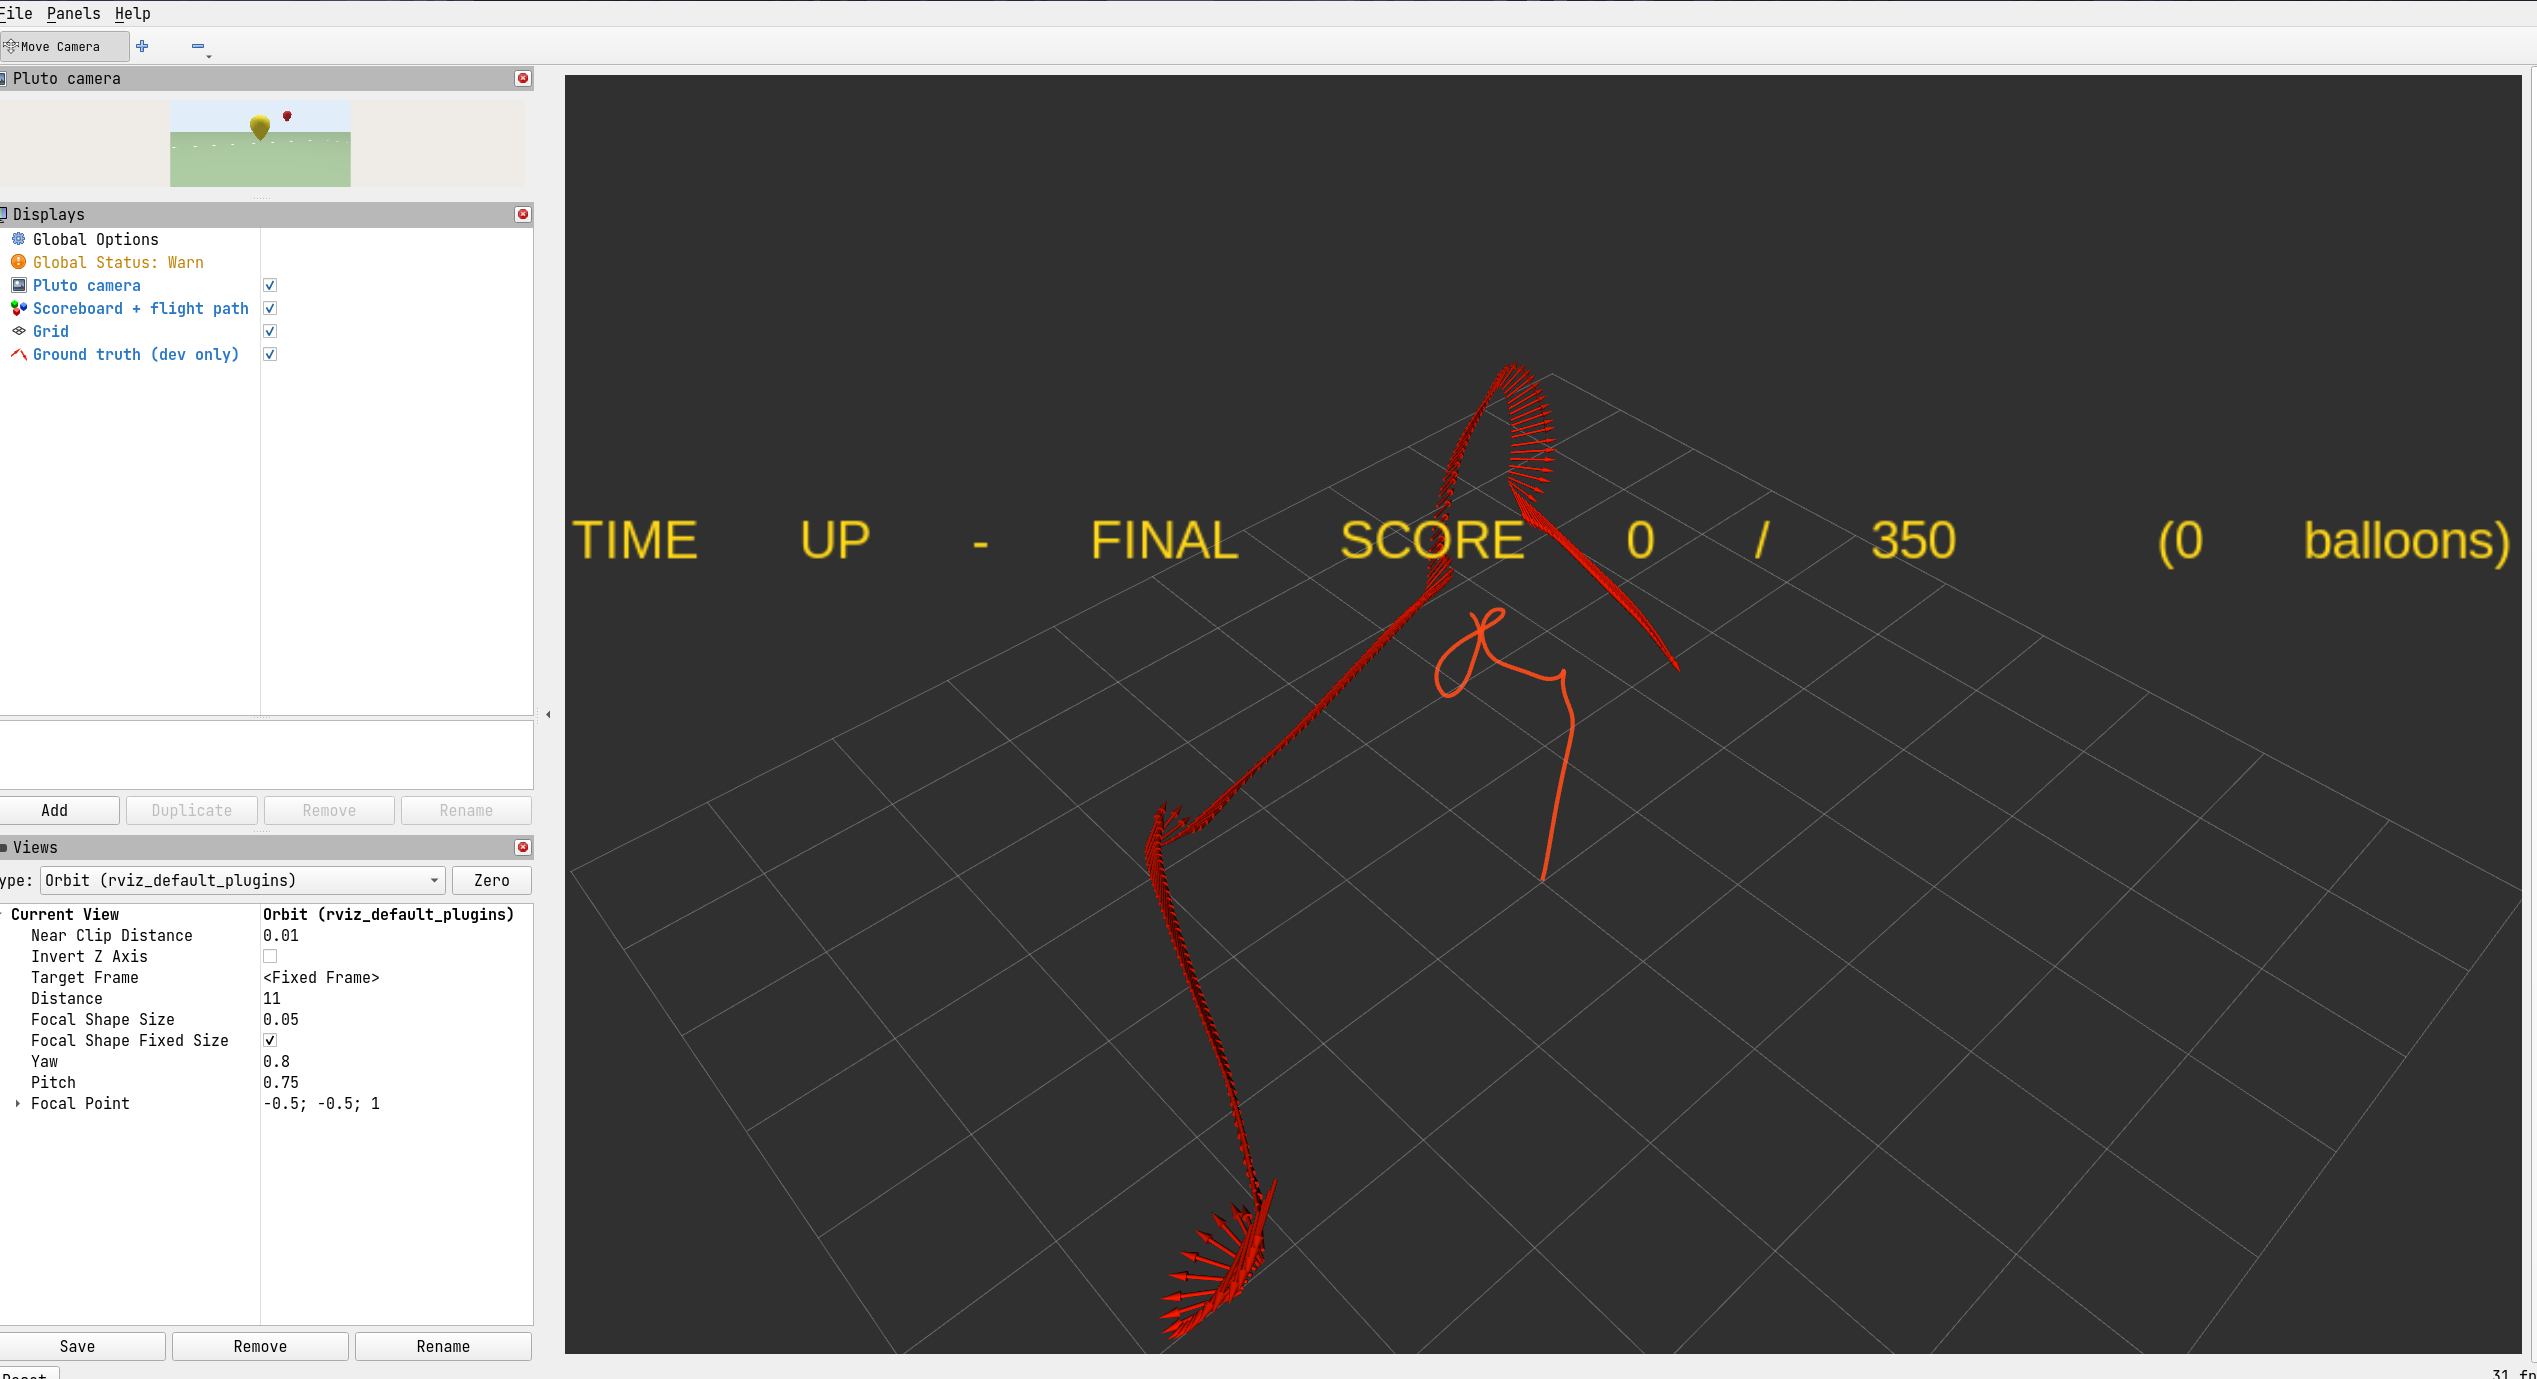
\includegraphics[width=\linewidth]{figures/rviz.png}\\
    {\scriptsize RViz: the drone's camera, its path, the score}
  \end{columns}
\end{frame}

% ===========================================================================
\section{Rounds and deadlines}
\begin{frame}{Rounds, deadlines and expectations}
  \begin{columns}[T]
    \column{0.49\textwidth}
    \begin{block}{Round 1: Simulation}
      \small
      Opens: \textbf{\RoundOneOpens} \quad Deadline: \textbf{\RoundOneDeadline}\\[1mm]
      Submit \textbf{all} of:
      \begin{enumerate}\small
        \item your controller: \code{outerloop\_controller/}
        \item the \textbf{analysis notebook} of your best run, executed
        \item the \textbf{evaluation notebook}, executed ($\geq$10 runs)
        \item a \textbf{video} of your best run (Gazebo + RViz)
        \item a \textbf{report}: your outer-loop idea, what worked,
              what did not
      \end{enumerate}
      Judged on layouts \textbf{you have not seen}.
    \end{block}
    \column{0.49\textwidth}
    \begin{block}{Round 2: Hardware}
      \small
      Shortlist: \textbf{\ShortlistDate} \quad Round: \textbf{\RoundTwoDate}\\[1mm]
      \begin{itemize}\small
        \item The top teams of Round 1 are invited.
        \item The \textbf{same program} flies the real Pluto X
              (\code{--hardware}).
        \item Real video delay, real lighting, a real battery.
        \item Time to test and tune on site before the scored flights.
        \item The judges count the balloons.
      \end{itemize}
    \end{block}
  \end{columns}
\end{frame}

% ===========================================================================
\section{The simulation}
\begin{frame}[fragile]{Setup in three steps}
  \begin{enumerate}
    \item \textbf{Clone} the repository
    \item \textbf{Choose} how to run it:
      \begin{itemize}
        \item \textbf{Docker dev container} (recommended; Linux, Windows via WSL2, macOS):
              VS Code $\rightarrow$ \textit{Dev Containers: Reopen in Container}
        \item \textbf{Local} (Ubuntu 22.04 only): install ROS 2 Humble and
              Gazebo Harmonic, then \code{colcon build}
      \end{itemize}
    \item \textbf{Fly} the example
  \end{enumerate}
  \vspace{2mm}
  \begin{columns}[c]
    \column{0.58\textwidth}
\begin{semiverbatim}\scriptsize
git clone --recursive https://\RepoURL.git
cd AVATIC
# (local setup only: source /opt/ros/humble/setup.bash
#                    && colcon build
#                    && source install/setup.bash)
ros2 launch pluto_x_bringup competition.launch.py \textbackslash
  controller:=outerloop_controller/examples/hello_drone.py
\end{semiverbatim}
    \column{0.4\textwidth}\centering
    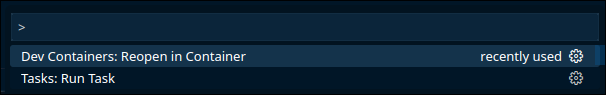
\includegraphics[width=\linewidth]{figures/reopen.png}\\
    {\scriptsize VS Code: open the dev container}
  \end{columns}
  \vspace{1mm}
  {\scriptsize Step-by-step instructions for every operating system: \code{workshop/manual.md} in the repository.}
\end{frame}

\begin{frame}{How it fits together: two control loops}
  \centering
  \resizebox{0.98\linewidth}{!}{%
  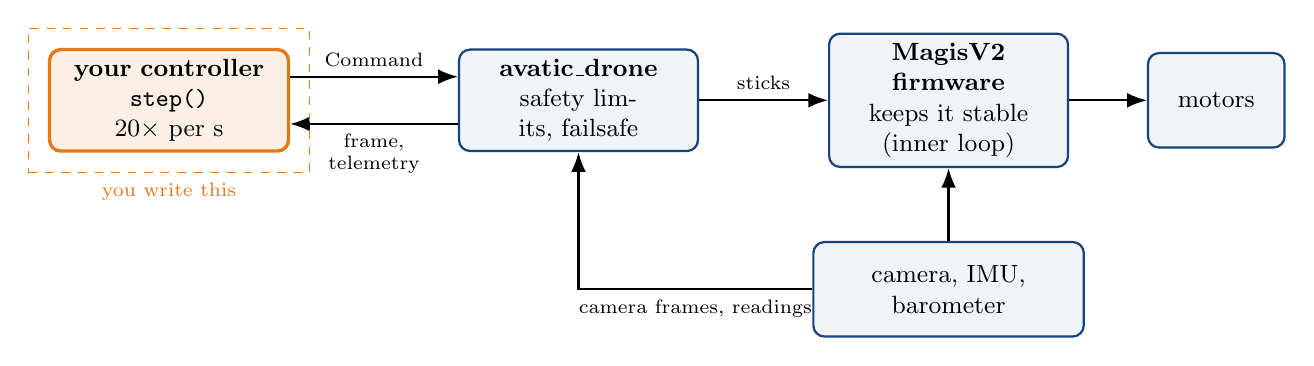
\begin{tikzpicture}[
      blk/.style={draw=avBlue,thick,rounded corners,fill=avBlue!6,align=center,
                  minimum height=1.2cm,text width=2.8cm,font=\small},
      you/.style={blk,draw=avAccent,fill=avAccent!12,very thick},
      arr/.style={-{Latex[length=2.5mm]},thick}]
    \node[you] (ctrl) at (0,0) {\textbf{your controller}\\ \code{step()}\\ 20$\times$ per s};
    \node[blk] (api) at (5.2,0) {\textbf{avatic\_drone}\\ safety limits, failsafe};
    \node[blk] (fc) at (9.9,0) {\textbf{MagisV2 firmware}\\ keeps it stable\\ (inner loop)};
    \node[blk,text width=1.5cm] (mot) at (13.3,0) {motors};
    \node[blk,text width=3.2cm] (sens) at (9.9,-2.4) {camera, IMU, barometer};
    \draw[arr] ([yshift=3mm]ctrl.east) -- node[above,font=\scriptsize]{Command} ([yshift=3mm]api.west);
    \draw[arr] ([yshift=-3mm]api.west) -- node[below,font=\scriptsize,align=center]{frame,\\ telemetry} ([yshift=-3mm]ctrl.east);
    \draw[arr] (api) -- node[above,font=\scriptsize]{sticks} (fc);
    \draw[arr] (fc) -- (mot);
    \draw[arr] (sens) -- (fc);
    \draw[arr] (sens.west) -| node[below,pos=0.25,font=\scriptsize]{camera frames, readings} (api.south);
    \node[draw=avAccent,dashed,fit=(ctrl),inner sep=2.5mm,
          label={[font=\scriptsize,text=avAccent]below:you write this}] {};
  \end{tikzpicture}}\\[3mm]
  \small The \textbf{inner loop} (firmware) holds the tilt and turn rate you ask for.
  The \textbf{outer loop} (you) decides where to go, from the camera.
\end{frame}

\begin{frame}[fragile]{What you get, and what you write}
  \begin{columns}[T]
    \column{0.52\textwidth}
    \begin{block}{Given to you}
      \small
      \begin{itemize}
        \item \code{my\_controller.py}: template that takes off and hovers
        \item \code{avatic\_drone}: the drone interface (sim and real)
        \item \code{hello\_drone.py}: example using the camera and commands
        \item \textbf{demo}: a pre-planned route popping every good balloon (fixed layout)
        \item \textbf{analysis}: every run recorded + a notebook
        \item \textbf{evaluation}: test on many hidden-style layouts
        \item the participant guide (\code{docs/participants/})
      \end{itemize}
    \end{block}
    \column{0.46\textwidth}
    \begin{alertblock}{You write}
      \small
      \code{MyController.step()} in\\ \code{outerloop\_controller/my\_controller.py}
\begin{semiverbatim}\scriptsize
def step(self, frame, telemetry, t):
    # frame:     camera picture
    # telemetry: tilt, heading,
    #            height, battery
    # t:         seconds since arming
    ...
    return Command(roll=0.0,
                   pitch=0.0,
                   yaw\_rate=0.0,
                   throttle=0.76)
\end{semiverbatim}
      Plain Python (NumPy, OpenCV). No ROS needed.
    \end{alertblock}
  \end{columns}
\end{frame}

\begin{frame}{Commands and readings}
  \begin{columns}[T]
    \column{0.52\textwidth}
    \textbf{You send} (\code{Command})\\[1mm]
    \scriptsize
    \begin{tabularx}{\linewidth}{@{}l l X@{}}
      \toprule
      & range & meaning \\
      \midrule
      \code{roll} & $-1\ldots1$ & tilt right (+): slides right; 0.2 $\approx$ 7°, max 20° \\
      \code{pitch} & $-1\ldots1$ & nose down (+): flies forward \\
      \code{yaw\_rate} & $-1\ldots1$ & turn clockwise (+), $\approx$77°/s per unit \\
      \code{throttle} & $0\ldots1$ & lift; \textbf{$\approx$0.76 hovers} \\
      \bottomrule
    \end{tabularx}\\[2mm]
    \normalsize\textbf{Safety limits} (sim and real)\\
    \scriptsize tilt $\leq$0.6, yaw rate $\leq$0.8, throttle $\leq$0.95; above
    2.5\,m it comes down; no command for 0.5\,s $\Rightarrow$ it levels itself.
    \column{0.46\textwidth}
    \textbf{You read} (\code{telemetry})\\[1mm]
    \scriptsize
    \begin{tabularx}{\linewidth}{@{}l X@{}}
      \toprule
      \code{altitude\_m} & height, from the barometer \\
      \code{heading\_deg} & 0 = north, 90 = east (start), clockwise \\
      \code{roll\_deg} & + = right side down \\
      \code{pitch\_deg} & + = nose up \\
      \code{battery\_v} & battery voltage \\
      \code{armed} & motors running \\
      \bottomrule
    \end{tabularx}\\[2mm]
    \normalsize\textbf{No position, no speed}\\
    \scriptsize like the real drone: the camera is your main sensor.
  \end{columns}
\end{frame}

\begin{frame}{The camera}
  \begin{columns}[c]
    \column{0.52\textwidth}
    \small
    \begin{itemize}
      \item 1280 $\times$ 720 RGB, about 18 frames/s, 80° $\times$ 50° view
      \item under the nose, looking ahead: \textbf{it tilts with the drone}
      \item mount: 3.5\,cm forward, 1.8\,cm below the centre
      \item pinhole model, no distortion:
            $K = \left[\begin{smallmatrix} 762.7 & 0 & 640\\ 0 & 762.7 & 360\\ 0&0&1 \end{smallmatrix}\right]$
      \item direction to a pixel $u$:\\ bearing $= \arctan\big((u-640)/762.7\big)$
      \item distance to a balloon (30\,cm wide):\\ $d \approx 229\,/\,\text{width in pixels}$ metres
    \end{itemize}
    \column{0.46\textwidth}\centering
    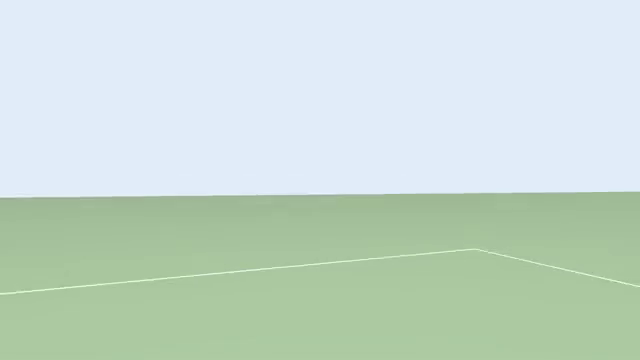
\includegraphics[width=0.66\linewidth]{figures/cam_search.png}\\[-0.5mm]
    {\scriptsize searching (turning on the spot)}\\[1.5mm]
    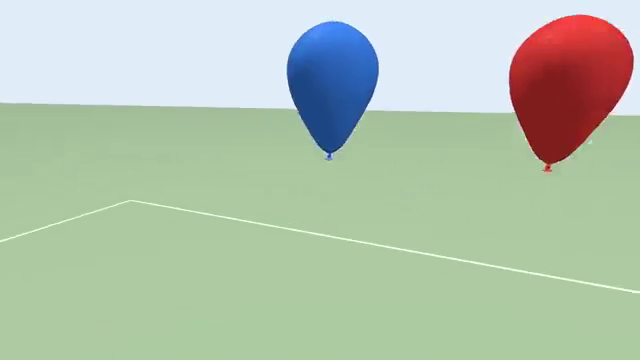
\includegraphics[width=0.66\linewidth]{figures/cam_approach.png}\\[-0.5mm]
    {\scriptsize a target in view (blue), a red one to avoid}
  \end{columns}
\end{frame}

\begin{frame}[fragile]{Running the simulator}
\begin{semiverbatim}\scriptsize
ros2 launch pluto_x_bringup competition.launch.py controller:=outerloop_controller/my_controller.py
\end{semiverbatim}
  \vspace{-1mm}
  \scriptsize
  \renewcommand{\arraystretch}{1.1}
  \begin{tabularx}{\linewidth}{@{}l X l@{}}
    \toprule
    \textbf{Option} (\code{name:=value}) & \textbf{what it does} & \textbf{default} \\
    \midrule
    \code{controller:=<file>} & the controller to run (any path) & none \\
    \code{headless:=true} & no Gazebo window: faster & \code{false} \\
    \code{rviz:=false} & no RViz window & \code{true} \\
    \code{arena\_seed:=random} / \code{:=7} & a random / a specific balloon layout & development layout \\
    \code{time\_limit\_s:=30} & longer runs while developing (judging: 15) & \code{15} \\
    \code{record:=false} & do not save this run & \code{true} \\
    \code{record\_dir:=<folder>} & save runs elsewhere & \code{analysis/runs} \\
    \bottomrule
  \end{tabularx}\\[2mm]
  \normalsize
  \begin{columns}[T]
    \column{0.5\textwidth}
    \small\textbf{Other commands}
    \begin{itemize}\scriptsize
      \item demo: \code{ros2 launch pluto\_x\_demo balloon\_demo.launch.py}
      \item new practice layout: \code{python3 analysis/new\_seed.py}
    \end{itemize}
    \column{0.48\textwidth}
    \small\textbf{Good to know}
    \begin{itemize}\scriptsize
      \item one run per launch: Ctrl-C, then start again
      \item every run is saved automatically
    \end{itemize}
  \end{columns}
\end{frame}

\begin{frame}{Analysis: understand one flight}
  \begin{columns}[c]
    \column{0.42\textwidth}
    \small
    \begin{itemize}
      \item Every run is saved in \code{analysis/runs/}
      \item Open \code{analysis/analysis.ipynb}, run all cells
      \item Your \textbf{score} first, then:
        \begin{itemize}\scriptsize
          \item a map of the flight over the balloons
          \item height, distance to every balloon
          \item your commands over time
          \item camera pictures at key moments
        \end{itemize}
      \item The map uses the \textbf{true} position: your controller
            never gets it, but you can learn from it
    \end{itemize}
    \column{0.56\textwidth}\centering
    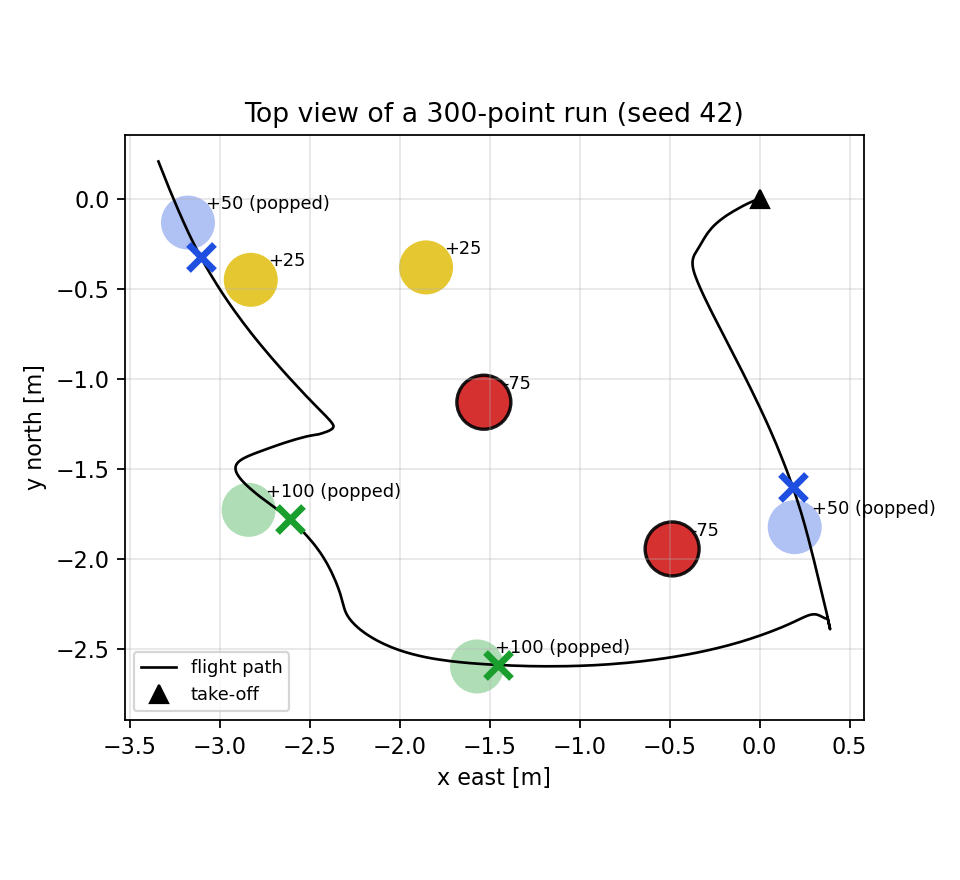
\includegraphics[width=0.9\linewidth]{figures/run_map.png}
  \end{columns}
\end{frame}

\begin{frame}{Analysis: what happened, over time}
  \centering
  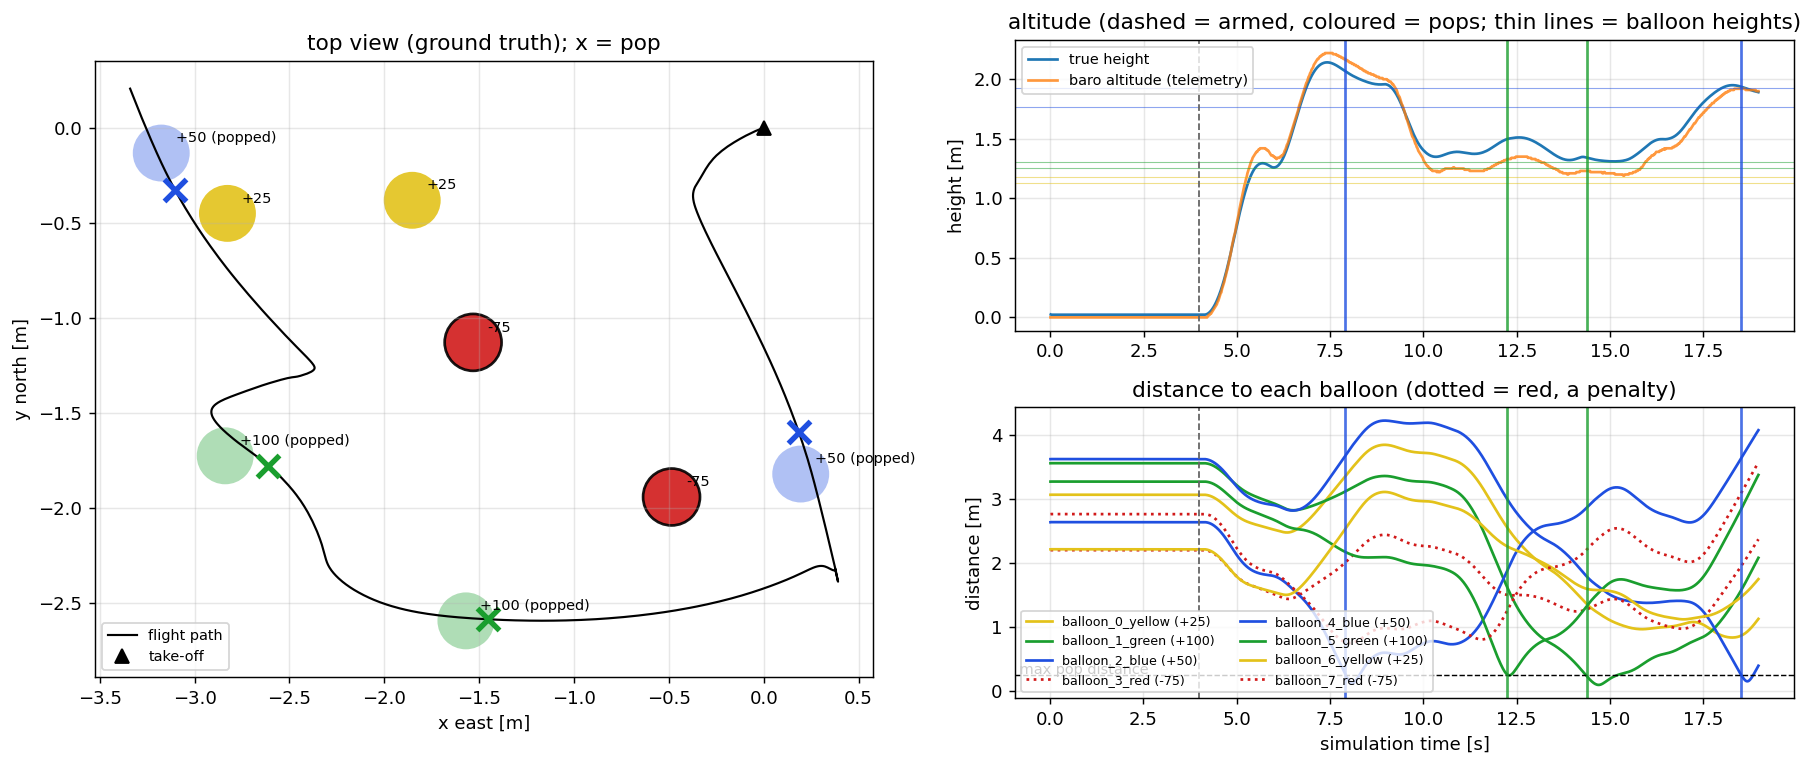
\includegraphics[width=0.97\linewidth,height=0.72\textheight,keepaspectratio]{figures/run_overview.png}\\
  \small Top view, height, and the distance to each balloon (dotted: red). Did you get close to the one you wanted?
\end{frame}

\begin{frame}[fragile]{Evaluation: test like the judges}
  \begin{columns}[c]
    \column{0.45\textwidth}
    \small
\begin{semiverbatim}\scriptsize
python3 evaluation/evaluate.py \textbackslash
  --controller \textbackslash
    outerloop_controller/my_controller.py \textbackslash
  --runs 10
\end{semiverbatim}
    \begin{itemize}
      \item 10 runs on 10 \textbf{random layouts}, no windows
            (about 25\,s each)
      \item then \code{evaluation/evaluation.ipynb}:
            \textbf{average score}, worst and best run, red hits,
            balloons per colour
      \item a controller that never arms scores 0
      \item runs vary: judge a change over several runs
    \end{itemize}
    \column{0.53\textwidth}\centering
    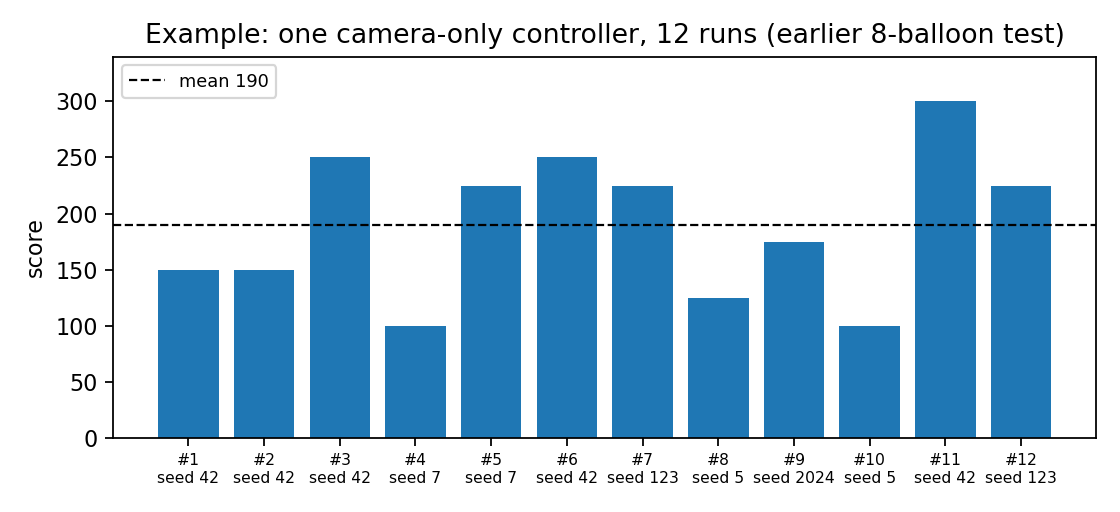
\includegraphics[width=\linewidth]{figures/example_scores.png}\\
    {\scriptsize A camera-only test controller: scores vary a lot between layouts}
  \end{columns}
\end{frame}

% ===========================================================================
\section{Solution ideas}
\begin{frame}{Solution ideas: a pipeline, not a solution}
  \centering
  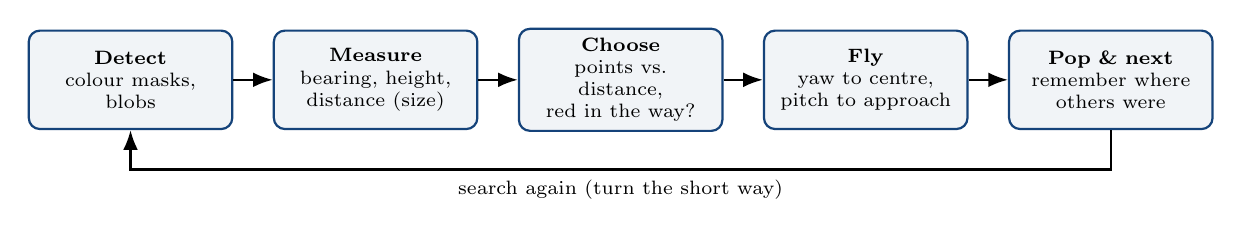
\begin{tikzpicture}[
      st/.style={draw=avBlue,thick,rounded corners,fill=avBlue!6,align=center,
                 minimum height=1.25cm,text width=2.35cm,font=\scriptsize},
      arr/.style={-{Latex[length=2.5mm]},thick}]
    \node[st] (a) {\textbf{Detect}\\ colour masks,\\ blobs};
    \node[st,right=5mm of a] (b) {\textbf{Measure}\\ bearing, height,\\ distance (size)};
    \node[st,right=5mm of b] (c) {\textbf{Choose}\\ points vs.\ distance,\\ red in the way?};
    \node[st,right=5mm of c] (d) {\textbf{Fly}\\ yaw to centre,\\ pitch to approach};
    \node[st,right=5mm of d] (e) {\textbf{Pop \& next}\\ remember where\\ others were};
    \draw[arr] (a)--(b); \draw[arr] (b)--(c); \draw[arr] (c)--(d); \draw[arr] (d)--(e);
    \draw[arr] (e.south) -- ++(0,-0.5) -| node[below,pos=0.25,font=\scriptsize]{search again (turn the short way)} (a.south);
  \end{tikzpicture}\\[5mm]
  \begin{columns}[T]
    \column{0.49\textwidth}
    \small
    \begin{itemize}
      \item Structure it as a \textbf{state machine}: take off $\rightarrow$
            search $\rightarrow$ approach $\rightarrow$ pop $\rightarrow$ \ldots
      \item Work on a \textbf{smaller image} (\code{image[::4, ::4]}) for speed
      \item A \textbf{proportional} yaw on the pixel offset is a good start
    \end{itemize}
    \column{0.49\textwidth}
    \small
    \begin{itemize}
      \item Go for \textbf{green} first: 100 vs.\ 25 points
      \item Check the path for \textbf{red} before pushing forward
      \item Use the heading to \textbf{remember} balloons you have seen
    \end{itemize}
  \end{columns}
\end{frame}

\begin{frame}{Solution ideas: the hard parts}
  \begin{columns}[c]
    \column{0.55\textwidth}
    \small
    \begin{itemize}
      \item \textbf{Drift.} There is no speed reading. If a balloon keeps
            sliding sideways in the picture, you are drifting: correct
            with roll.
      \item \textbf{Momentum.} The drone keeps its speed: brake before
            you arrive.
      \item \textbf{Time.} A full turn takes $\approx$6\,s of your 15\,s.
            Plan the search.
      \item \textbf{The camera tilts} with the drone: pitching forward
            moves the scene up in the picture.
      \item \textbf{Throttle}: change it smoothly, never cut it in the air.
      \item \textbf{Real video is late} (0.15--0.4\,s): smooth beats fast.
    \end{itemize}
    \column{0.43\textwidth}\centering
    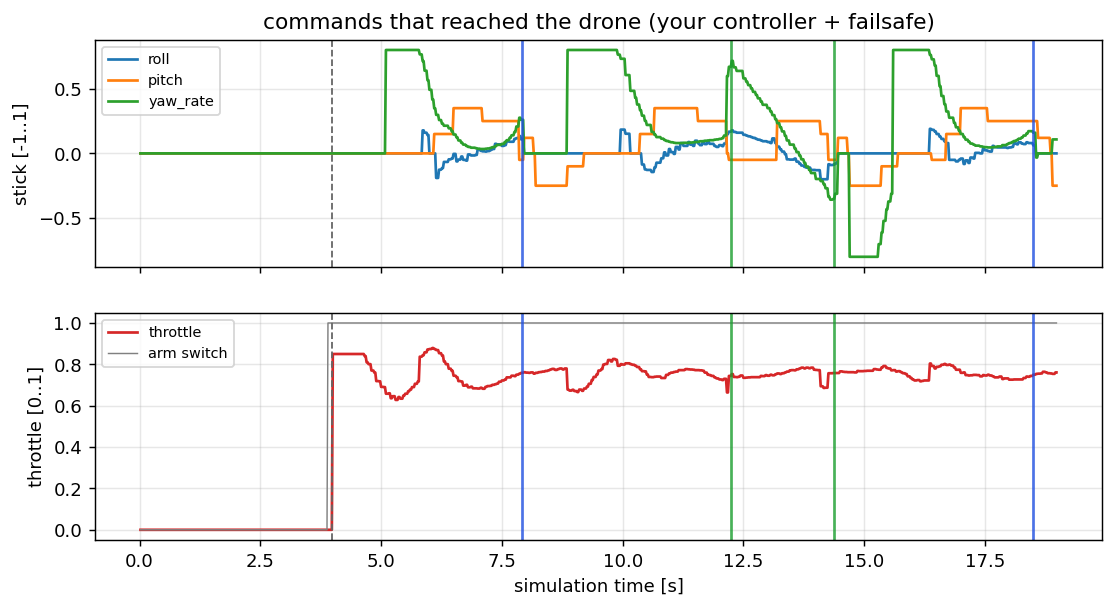
\includegraphics[width=\linewidth]{figures/run_commands.png}\\
    {\scriptsize Commands of the 300-point run}
  \end{columns}
\end{frame}

% ===========================================================================
\section{Sim2real}
\begin{frame}[fragile]{Sim2real: the same program on the real Pluto X}
  \centering
  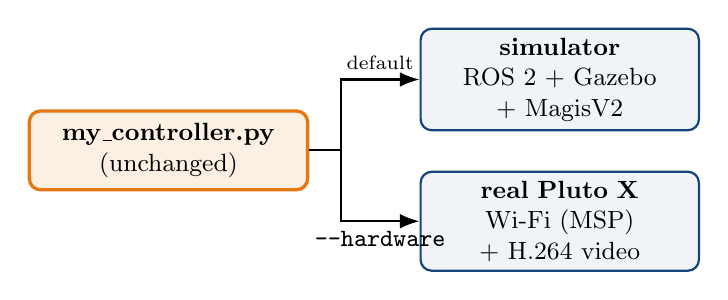
\begin{tikzpicture}[
      blk/.style={draw=avBlue,thick,rounded corners,fill=avBlue!6,align=center,
                  minimum height=1cm,text width=3.3cm,font=\small},
      you/.style={blk,draw=avAccent,fill=avAccent!12,very thick},
      arr/.style={-{Latex[length=2.5mm]},thick}]
    \node[you] (c) {\textbf{my\_controller.py}\\ (unchanged)};
    \node[blk,right=14mm of c,yshift=9mm] (s) {\textbf{simulator}\\ ROS 2 + Gazebo\\ + MagisV2};
    \node[blk,right=14mm of c,yshift=-9mm] (h) {\textbf{real Pluto X}\\ Wi-Fi (MSP)\\ + H.264 video};
    \draw[arr] (c.east) -- ++(4mm,0) |- node[above,pos=0.75,font=\scriptsize]{default} (s.west);
    \draw[arr] (c.east) -- ++(4mm,0) |- node[below,pos=0.75,font=\scriptsize]{\code{--hardware}} (h.west);
  \end{tikzpicture}\\[3mm]
\begin{semiverbatim}\small
python3 outerloop_controller/my_controller.py --hardware
\end{semiverbatim}
  \vspace{-2mm}
  \begin{columns}[T]
    \column{0.49\textwidth}
    \small\textbf{The same on both}
    \begin{itemize}\scriptsize
      \item the same commands, readings and sign conventions
      \item the same firmware and safety limits
      \item landing at the end, Ctrl-C = land, twice = motors off
    \end{itemize}
    \column{0.49\textwidth}
    \small\textbf{Different on the real drone}
    \begin{itemize}\scriptsize
      \item video delay, fewer frames per second
      \item real lighting: re-tune your colour ranges
      \item hover throttle depends on the drone and battery
      \item no scoreboard: the judges count
    \end{itemize}
  \end{columns}
\end{frame}

\begin{frame}{Sim2real: how to prepare}
  \begin{columns}[c]
    \column{0.55\textwidth}
    \begin{enumerate}\small
      \item \textbf{Be robust in simulation}: good average over many
            random layouts, not one lucky run
      \item \textbf{Don't rely on exact numbers}: colours, sizes and
            timings will change
      \item \textbf{Design for delay}: slow, smooth commands; don't
            react to a single frame
      \item \textbf{Make thresholds easy to change}: keep them at the top
            of your file
      \item \textbf{On site}: collect a few real camera frames first,
            check colours and hover throttle, then fly
      \item \textbf{Safety first}: Ctrl-C to land, keep people clear
    \end{enumerate}
    \column{0.43\textwidth}\centering
    \figOrBox{figures/arena_real.jpg}{\linewidth}{photo of the real arena\\(to be added)}
  \end{columns}
\end{frame}

% ===========================================================================
\section{Deadlines}
\begin{frame}{Deadlines}
  \centering
  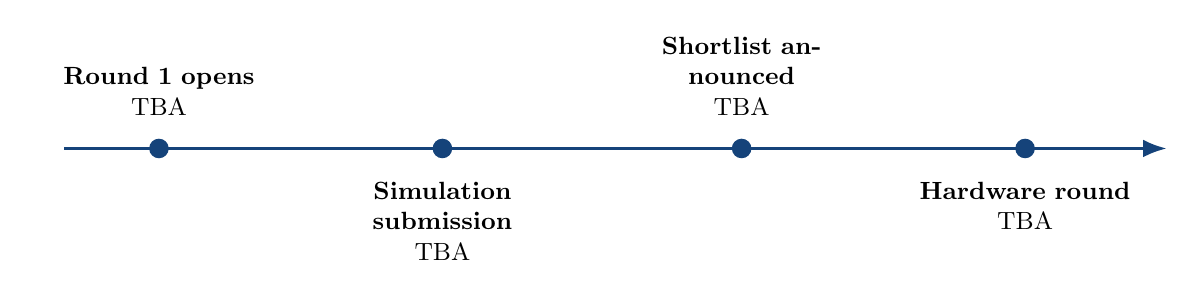
\begin{tikzpicture}[
      ev/.style={circle,fill=avBlue,inner sep=2.5pt},
      lab/.style={align=center,font=\small,text width=3.1cm}]
    \draw[very thick,avBlue,-{Latex[length=3mm]}] (0,0) -- (14,0);
    \foreach \x/\name/\date/\pos in {
        1.2/Round 1 opens/\RoundOneOpens/above,
        4.8/Simulation submission/\RoundOneDeadline/below,
        8.6/Shortlist announced/\ShortlistDate/above,
        12.2/Hardware round/\RoundTwoDate/below} {
      \node[ev] at (\x,0) {};
      \node[lab,\pos=3mm] at (\x,0) {\textbf{\name}\\ \date};
    }
  \end{tikzpicture}\\[8mm]
  \begin{alertblock}{Submission (Round 1)}
    \small controller code \quad+\quad executed analysis notebook (best run)
    \quad+\quad executed evaluation notebook \quad+\quad video \quad+\quad report
  \end{alertblock}
\end{frame}

% ===========================================================================
\section{Prizes}
\begin{frame}{Prizes}
  \centering
  \vspace{8mm}
  {\Huge \faTrophy}\\[6mm]
  {\LARGE Prize pool: \textbf{\PrizePool}}\\[8mm]
  \small Details will be announced before the simulation deadline.
\end{frame}

% ===========================================================================
\section{Questions}
\begin{frame}{Get started today}
  \begin{columns}[c]
    \column{0.55\textwidth}
    \begin{enumerate}
      \item Clone \textbf{\RepoURL}
      \item Follow \code{workshop/manual.md} for your system
      \item Fly \code{hello\_drone.py}, then open \code{my\_controller.py}
      \item Read the participant guide: \code{docs/participants/}
    \end{enumerate}
    \vspace{4mm}
    \begin{block}{Questions?}
      \faEnvelope[regular]\ \ \ContactName\\
      \small\texttt{\ContactMail}
    \end{block}
    \column{0.43\textwidth}\centering
    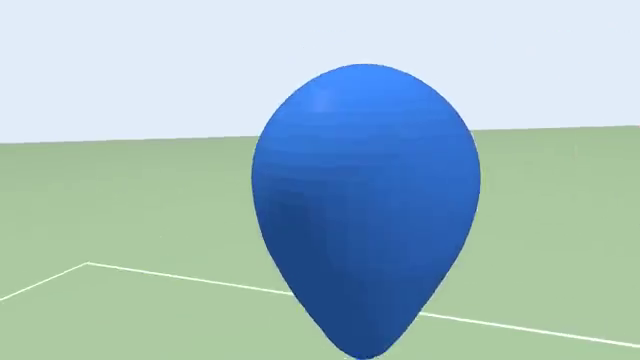
\includegraphics[width=\linewidth]{figures/cam_prepop.png}\\
    {\scriptsize Happy popping!}
  \end{columns}
\end{frame}

\end{document}
